\documentclass[technical_document.tex]{subfiles}
\begin{document}

Eva\textquotesingle{}s arm was designed with a focus on minimizing production time. %TODO reference design constrains from the paper?
Two independent 3D drawings were made using CAD software\footnote{Solidworks was used as the main CAD program for all mechanical parts}. These designs gave a good overview of the required parts and were helpful in estimating the production time. Realizing the production time was very limited\footnote{Just one month was planned as production time, to leave some time for testing}, the final design resulted from combining the two different designs in a way that would minimize production time.
Mostly this was done by dividing the arm into small parts that are easy to manufacture. This way even during a relatively short time (for example, if the workshop was only available for a few hours), a few parts could be made. Parts with wrong dimensions or other manufacturing errors could be replaced fairly quickly, as the production time per part is very low. 
These parts were created with more and more detail, in an iterative process. Parts that would be too complex were divided into smaller and simpler parts. In the CAD software these parts were connected to form the arm, including all necessary bolts and nuts. When all parts were finished, this main assembly was tested for interfering parts and possibility of assembling. Most parts are made from aluminium, since it is a lightweight and easily available material. Small shafts or connectors were mostly created from steel, since they generally have high stress concentrations on them. Furthermore, due to their small dimensions the extra weight is minimal. The assumptions about material choice have been validated using numerous calculations, as will be discussed later.

\section{Design of the arm}

Most important part of the robotic arm is the shoulder. It has to support the weight of the whole arm including the object in the gripper and should be strong and stiff enough for the gripper to be placed accurately, even when accelerating.

\begin{figure}[ht!]
	\centering
	\mbox{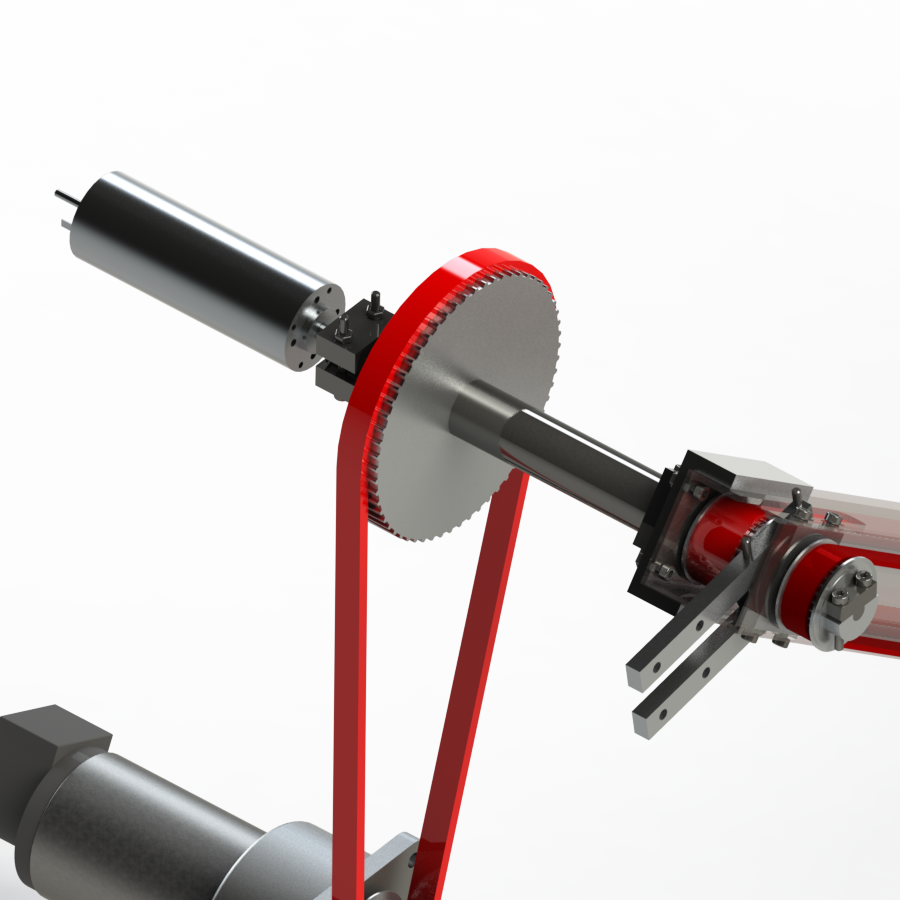
\includegraphics[scale=1.0]{Images/arm_shoulder.png}}
	\caption{Shoulder joint of Eva\textquotesingle{}s arm}
	\label{fig:arm_shoulder}
\end{figure}

The main idea is very simple. The upper arm is a standard square tube, connected to a hollow shaft. The shaft is supported by a set of bearings, resulting in an upper arm that can move freely in just one direction. The arm is moved by driving the shaft via a timing belt. There is a second motor located close to the shoulder, which drives the sideways motion of the arm. This is done via a small axis located within the main shoulder shaft, driving the lower arm via a set of timing belts. This second motor and especially its shaft running through the shoulder make this joint the most complex one. Another important thing to notice is the way the bearing mounts are connected to the upper arm. They are designed in such a way that just by re-tightening a few bolts, the tension on the belts can be adjusted.

From the shoulder to the elbow joint, the arm basically consists of a standard 40x40x2mm beam. The interesting part is how it links the elbow joint to the body. Inside the upper arm is another timing belt, connecting the elbow to a solid part of the shoulder. This ensures the lower arm is always in the same direction relative to the body. In this case the lower arm is always horizontal, as this is the most practical configuration for grasping objects from a table. Driving the inner timing belt with a motor instead of keeping it fixed to the body would make the lower arm capable of turning independently, adding another degree of freedom. This would be a relatively easy modification, as only a few changes are required in the shoulder. It would, however, make the arm slightly more difficult to control.

\begin{figure}[ht!]
	\centering
	\mbox{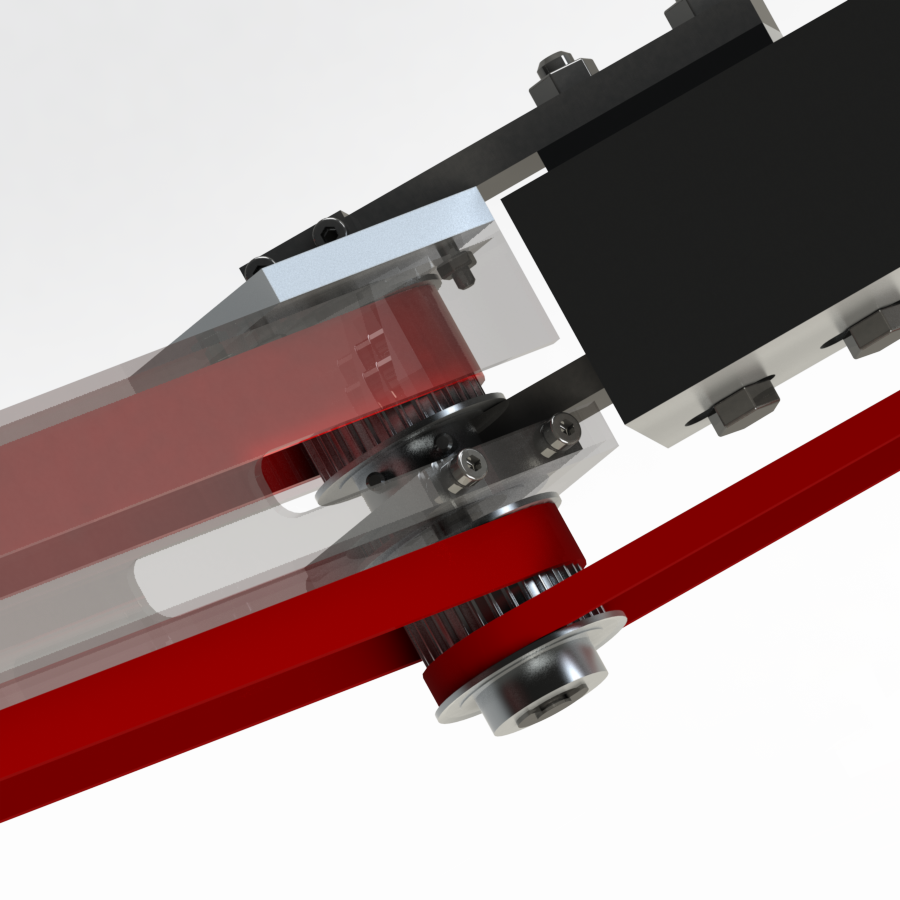
\includegraphics[scale=1.0]{Images/arm_elbow.png}}
	\caption{Elbow joint of Eva\textquotesingle{}s arm}
	\label{fig:arm_elbow}
\end{figure}

The elbow joint itself is fairly simple. The inner timing belt connects to a pulley, which is directly screwed onto the lower arm. This ensures the lower arm follows the reference angle given by the shoulder, as described earlier. The pulley is suspended by two bearings, connected to the upper arm via bearing mounts. Note these mounts are fixed in place, since the belt tension can be adjusted on the other end. The extra pulley on the outside of the joint is on the same shaft as the other pulley, but this one is free to turn independently of the shaft. The only purpose of this pulley is passing the rotation from the upper belt to the lower belt. This belt will eventually drive the sideways motion, as will be discussed in the next paragraph. The lower arm consists of the parts connected to the pulley and the beam itself. These are connected to each other in a way that allows adjusting the tension on the lower belt.

\begin{figure}[ht!]
	\centering
	\mbox{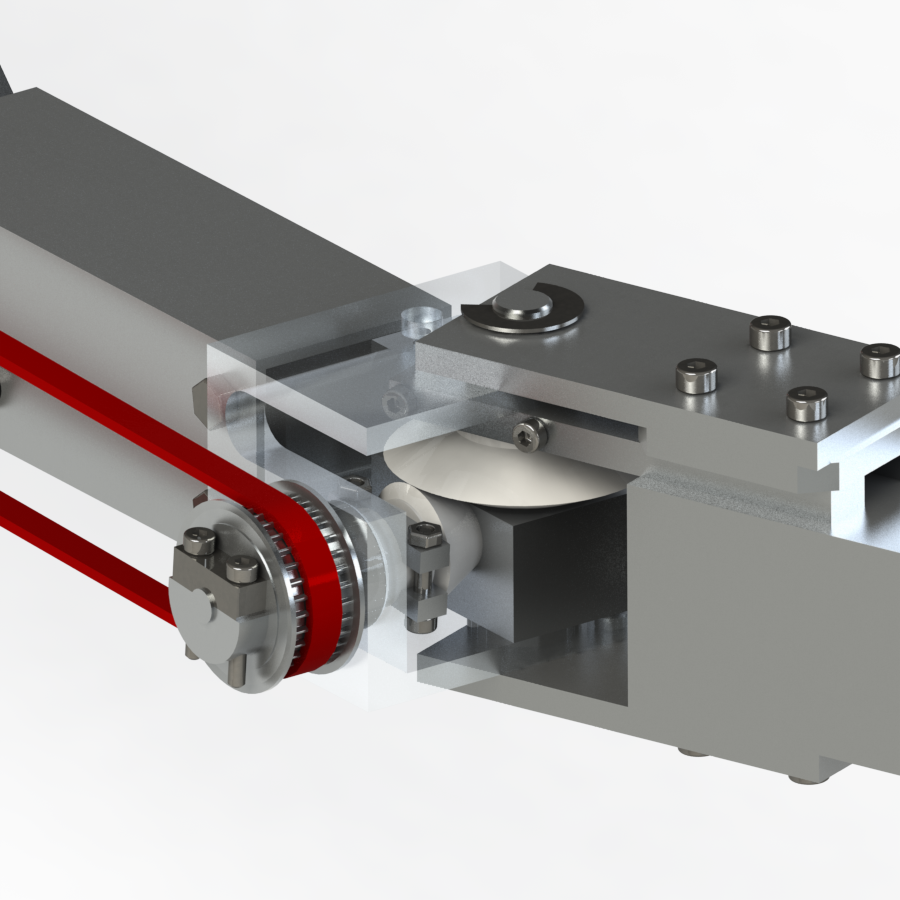
\includegraphics[scale=1.0]{Images/arm_sideJoint.png}}
	\caption{Sideways joint of Eva\textquotesingle{}s arm}
	\label{fig:arm_sideJoint}
\end{figure}

The last moving joint in the arm is the ‘sideJoint’: it allows Eva to move her arm a bit sideways. In a human arm, this direction of movement is integrated in the elbow, but Eva has a separate joint for this. The length of the link between those two joints is chosen based on the form of Eva’s body, so she can fold her arm in a compact way while driving or in standby mode. The motion is provided by the timing belt running on the outside of the arm. This belt drives a set of bevel gears to convert the rotation to the right direction. The bevel gears have a transmission ratio of 1:2, so the last link of the arm rotates with half the speed of the timing belt pulleys. This was done to makes the rotation less sensitive to play in the timing belts, lower the tension on the timing belts and simply because this set of gears is more compact than a comparable 1:1 set would be.

\begin{figure}[ht!]
	\centering
	\mbox{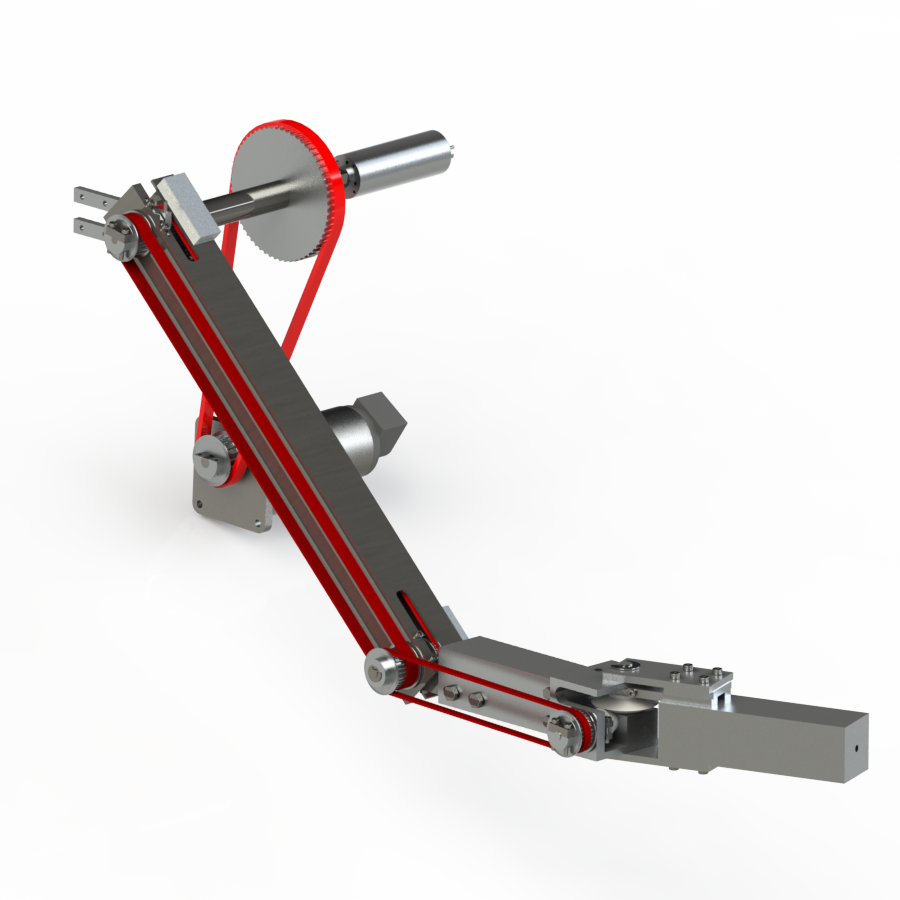
\includegraphics[scale=1.0]{Images/overview.png}}
	\caption{Overview of Eva\textquotesingle{}s arm}
	\label{fig:overview}
\end{figure}

The last part of the  arm is the gripper, connected to the ‘sideJoint’ via a standard beam. As the gripper design unfortunately is not open source, it was not possible to include it in our drawings. Linking all previously mentioned parts together, the total arm looks as in figure \ref{fig:overview}.


\section{strength calculations}

Before production, Eva\textquotesingle{}s arm was subjected to a number of calculations to check its strength and stiffness. The most critical point turned out to be the shoulder, as this is a complex part where a lot of torque concentrates. Furthermore, the upper arm needs to resist twisting as the lower arm is capable of moving sideways, potentially producing a significant torque on the upper arm. After numerous calculations, by hand as well as assisted by our CAD program, the conclusion was that most parts were  strong enough for our needs, but some needed reinforcement. Especially the upper arm would be too weak if made from aluminium. This is the reason the upper arm is made out of steel. Steel is a lot heavier than aluminium, but as the mass centre of this part is pretty close to the shoulder, its impact on the inertia is limited.
Including calculations with their according free-body diagrams and Solidworks simulations would be very verbose, as over 25 different parts have been designed, some of which are used multiple times in different situations. Therefore, only the most critical (thus the most interesting) parts of Eva’s arm are being discussed in this section.

\begin{figure}[ht!]
	\centering
	\mbox{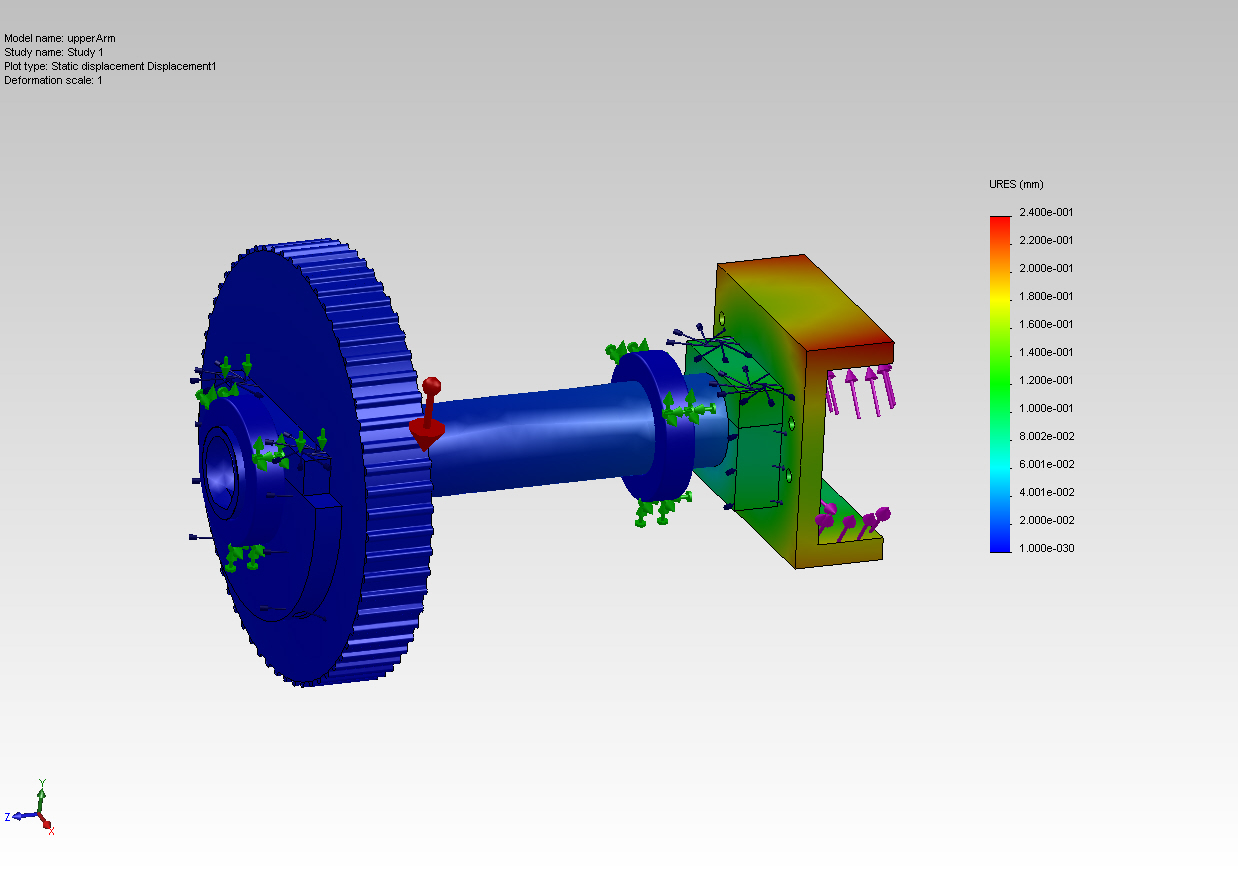
\includegraphics[scale=0.4]{Images/upperArm_displace.jpg}}
	\caption{Displacement plot of the shoulder}
	\label{fig:shoulder_displace}
\end{figure}

First point of interest was checking the shoulder mount. The weight of the arm and the object its grasps results in a torque around the shaft, as shown in \ref{fig:shoulder_displace} and fig.\ref{fig:shoulder_FOS}. The aluminium part connecting the arm with the shaft is the weakest point. Initially, this part was designed a bit too thin, resulting in large deformations and too much stress. Fig.\ref{fig:shoulder_displace} shows the deformation, where red is 0.2mm and blue is neutral. As expected, the corners displace the most from their original position, as a result of the torque. To see if the parts meet the strength requirements, a plot of the safety factor is shown in fig.\ref{fig:shoulder_FOS}

\begin{figure}[ht!]
	\centering
	\mbox{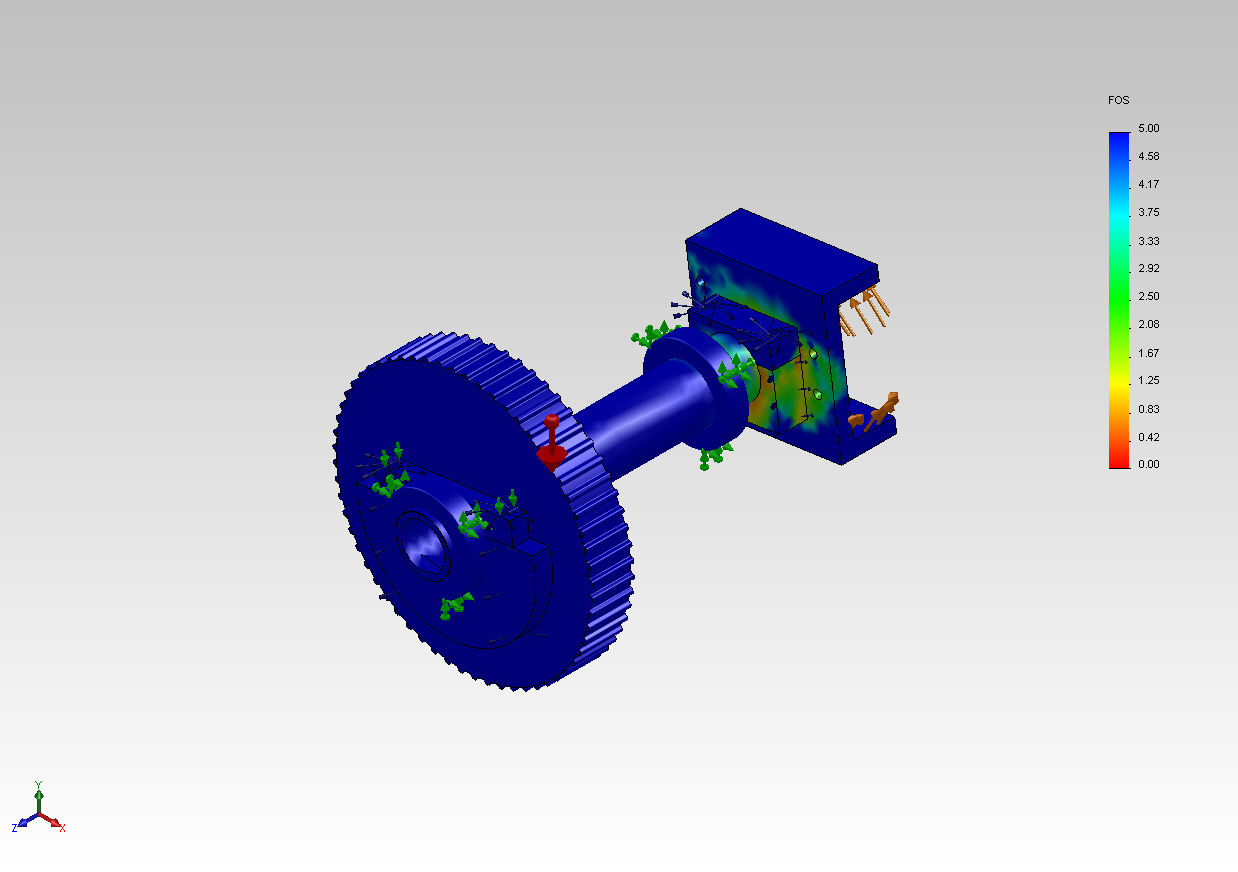
\includegraphics[scale=0.4]{Images/upperArm_FOS.jpg}}
	\caption{Factor of safety plot of the shoulder}
	\label{fig:shoulder_FOS}
\end{figure}

The factor of safety should be at least 1.0, as any value below indicates the part would probably break. The final design, as depicted in the figure, is strong enough. The factor of safety is generally above 5, but at some points it is around 1.0. These points are where all force concentrates on small areas or in close proximity of sharp corners.

Knowing the shoulder itself is strong enough, the upper arm is also of interest. Because of the large cuts in the arm, stress is expected to concentrate around its edges. The part was designed to be aluminium first, but the calculations showed it would be too weak. The beam in general is strong enough, but the edges of the cuts would certainly break. Its safety factor was below 0.5 and the stress was clearly higher than the aluminium would be able to take.Therefore steel was selected as material for the main beam of the upper arm. In fig.\ref{fig:upperArm_FOS} is the factor of safety plot, fig.\ref{fig:upperArm_displace} shows the deformation plot.

\begin{figure}[ht!]
	\centering
	\mbox{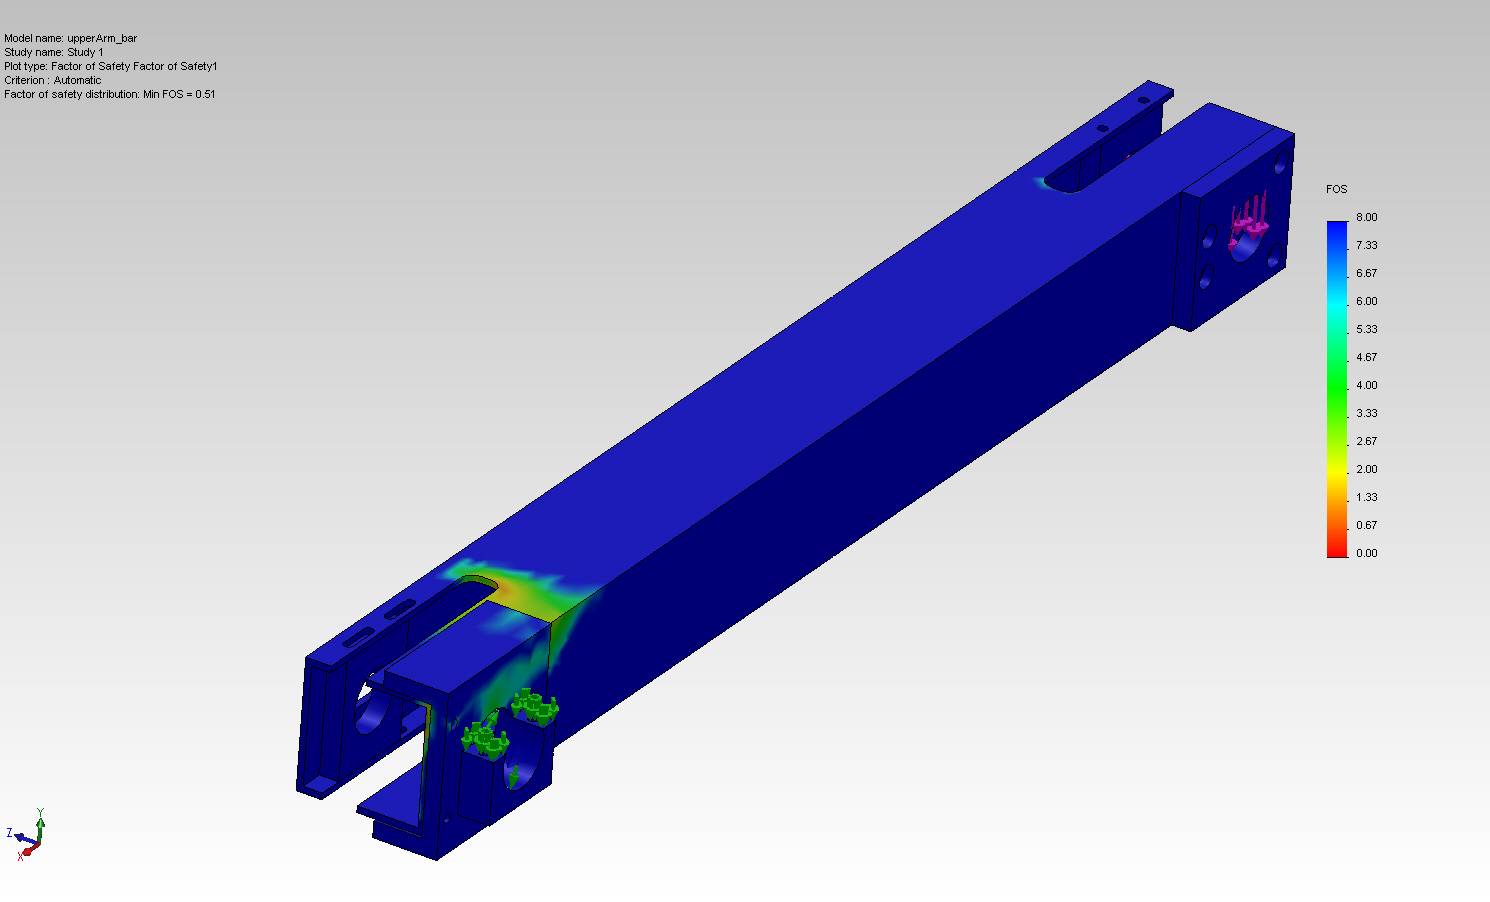
\includegraphics[scale=0.3]{Images/upperArm_bar_FOS.jpg}}
	\caption{Factor of safety plot of the upper arm}
	\label{fig:upperArm_FOS}
\end{figure}

Again it is clear that the main beam and the smaller bearing mounts are more than strong enough. However, at the edges of the slots in the main beam the safety factor decreases to almost 1. This is the reason steel was selected.

The deformation plot shows deformation up to 0.6mm, which is acceptable for our robot. If the arm could be designed without the slots it would be a lot less, and the arm could probably be made from aluminium. Because of time constrains it was decided to leave it this way, but it could be an improvement in a future version.

\begin{figure}[ht!]
	\centering
	\mbox{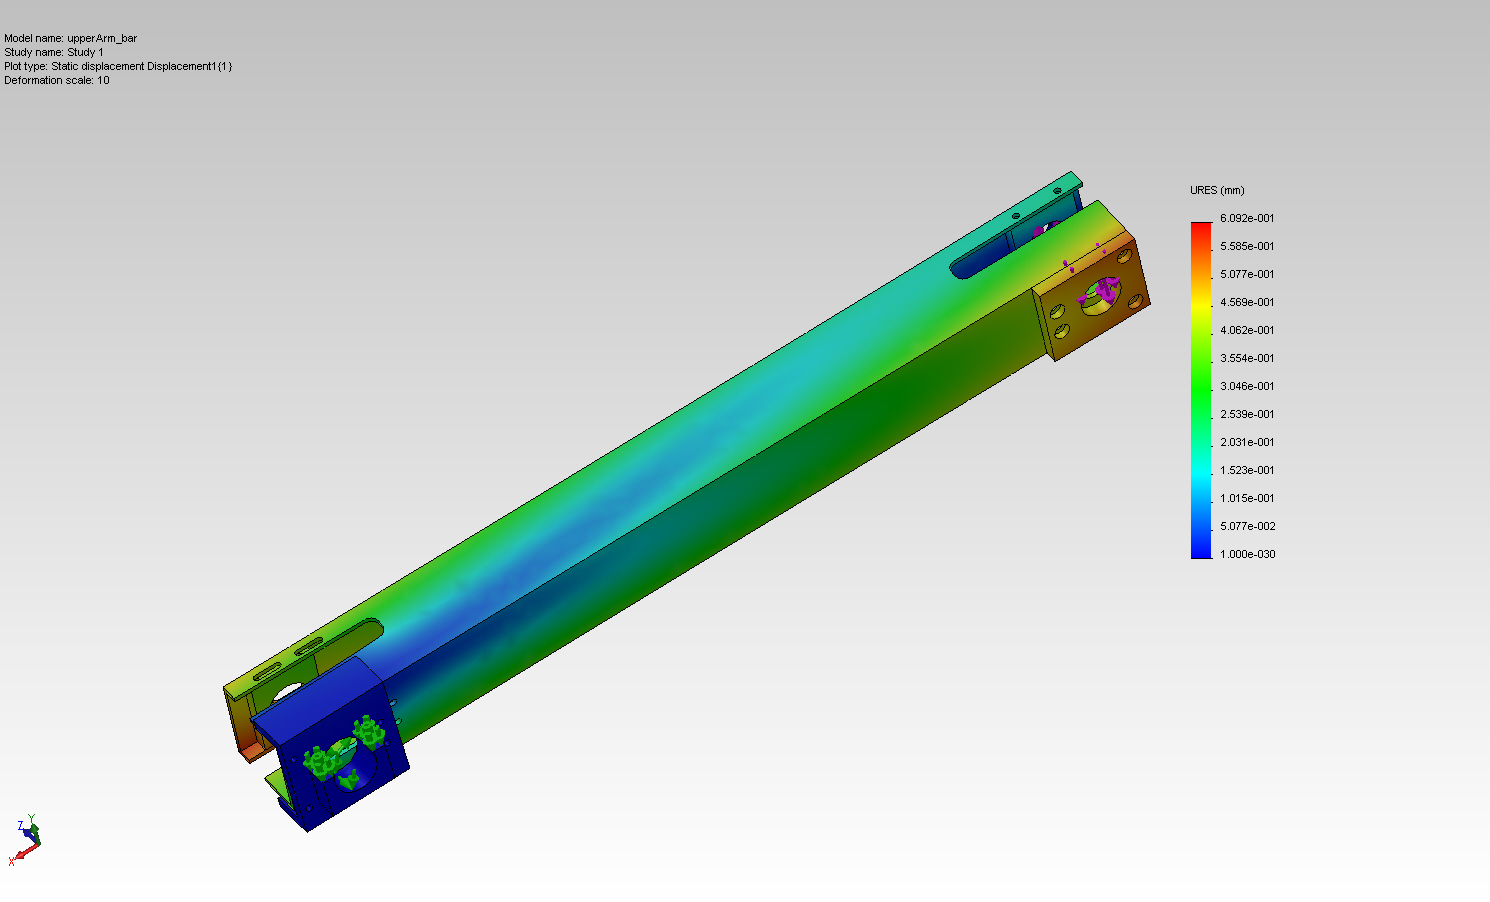
\includegraphics[scale=0.3]{Images/upperArm_bar_displace.jpg}}
	\caption{Displacement plot of the upper arm}
	\label{fig:upperArm_displace}
\end{figure}

These were the most important points. The further down the arm, the smaller the forces and the simpler the construction is. Most of those parts have been verified by simplified hand calculations. The main reason was time constrains. If one wishes to create a new version of Eva’s arm, doing more extensive calculations would be advisable. The arm certainly is strong enough, but it is probably possible to optimize its weight by removing redundant material.


\section{Motor choice}


 



\end{document}